\documentclass{school-22.211-notes}
\date{March  5, 2012}

\begin{document}
\maketitle

\clearpage
\topic{Heterogeneous Geometry Resonant Approximations}
This is probably the most important topic in generating cross section in reactor physics. We want to take into account both the spatial and energy structure distributions of flux within each resonance when solving the neutron slowing down problem. 

\begin{enumerate}
\item Assumptions for heterogeneous geometry resonant approximations:
\begin{itemize}
\item All neutron interactions in moderator are purely scattering;
\item Moderator scattering xs is independent of energy;
\item The previous two points together leads to that the slowing down energy source in fuel and moderator is 1/E;
\item Slowing down source is spatially uniform within each region (a fairly accurate assumption);
\item A single resonance absorber species exists only in the fuel;
\item Fuel scattering removes neutrons from resonance energy (that is, narrow resonance model); 
\end{itemize}

\item Spatial Reciprocity Theorem. First we introduce the reciprocity condition. The only assumption we make for this theorem is that the source is flat. This theorem does not depend on geometry. 

Given two homogeneous region 1 and 2, the probability of going from point A in 1 to point B in 2 without colliding is:
\eqn{ \frac{e^{-\tau}}{4 \pi R^2} }
where $\tau = \frac{x_1}{\lambda_1} + \frac{x_2}{\lambda_2} = x_1 \Sigma_1 + x_2 \Sigma_2$. The probability of going from A to B and then colliding at B is: 
\eqn{ \frac{e^{-\tau}}{4 \pi R^2} \Sigma_2 }
The probability of going from A to any point in region 2 and colliding is:
\eqn{ \int \frac{e^{-\tau}}{4 \pi R^2} \Sigma_2  \dV_2}
The probability of a uniform spatial neutron source in region 1 going to any point in region 2 and colliding is:
\eqn{ \int \dV_1 \int \frac{e^{-\tau}}{4 \pi R^2} \Sigma_2  \dV_2}
The average probability per unit volume of a uniform source neutron going from region 1 to 2 and colliding is:
\eqn{ P_{1\to 2} = \frac{\Sigma_2}{V_1} \int \dV_1 \int \frac{e^{-\tau}}{4 \pi R^2}  \dV_2}
Likewise,
\eqn{ P_{2\to 1} = \frac{\Sigma_1}{V_2} \int \dV_2 \int \frac{e^{-\tau}}{4 \pi R^2}  \dV_1}
Since the two integrals are symmetric (that is, $P_{A\to B}$ and $P_{B \to A}$ are essentially the same), we can write,
\eqn{ P_{1\to 2} \frac{V_1}{\Sigma_2} = P_{2\to 1} \frac{V_2}{\Sigma_1} }
Hence we reach the reciprocity condition:
\eqn{ \boxed{ P_{1\to 2} \Sigma_1 V_1 = P_{2\to 1} \Sigma_2 V_2 } }

\item Two Region Balance Equations. 
First collision reaction rate balance, where $\sigma_{t,f}(u) = \sigma_{r,f} + \sigma_{pot, f}$ (the resonance absorption xs plus the potential scattering xs):
\eqn{ \overbrace{N_f \sigma_{t,f} (u) \Phi(u) V_f}^{\mbox{fuel region lost neutrons}} = \overbrace{Q_f V_f P_{f\to f} + Q_m V_m P_{m\to f}}^{\mbox{fuel region gain neutrons from slowing down sources}}  }
Because slowing down sources in both fuel and moderator are assumed to arise from the 1/E flux above the resonance energy, we can write
\eqn{ Q_m &= N_m \sigma_{s,m} \Psi(u) &  Q_f&= N_f \sigma_{pot, f} \Psi(u) }
Plug the slowing down sources back into the reaction rate balance equation, and recall $\Phi(u) = \Psi(u) \phi(u)$ where $\phi(u)$ is the \hi{fine structure energy shape of the flux for homogeneous mixture}, we extand the definition to define $\phi_f(u)$ as the heterogeneous energy shape of flux in fuel,
\eqn{ N_f \sigma_{t,f} (u) \phi_f (u) V_f = N_f \sigma_{pot, f} V_f P_{f\to f} + N_m \sigma{s,m} V_m P_{m\to f} }
Next we use reciprocity relationship,
\eqn{ P_{m\to f} N_m \sigma_m V_m = P_{f\to m} N_f \sigma_f V_f}
and substitute into the balance equation to get,
\eqn{ N_f \sigma_{t}^F (u) \phi_f (u) V_f = N_f \sigma_{pot}^F V_f P_{f\to f} + N_f \sigma_{t}^F V_f P_{f\to m} }
Then we replace $P_{f\to m} = 1 - P_{f\to f}$ and get, 
\eqn{ N_f \sigma_{t}^F (u) \phi_f (u) V_f = N_f \sigma_{pot}^F V_f P_{f\to f} + N_f \sigma_{t}^F V_f (1 - P_{f\to f}) }
Divide both sides by the number of neutrons, we get a balance equation in unit of cross section:
\eqn{ \sigma_{t}^F (u) \phi_f (u) = \sigma_{pot}^F P_{f\to f} +  \sigma_{t}^F (1 - P_{f\to f}) }
That is, if we know $P_{f\to f}$, we can solve for the spatially averaged energy shape of the flux in the fuel. 

\item Wigner's Approximation of $P_{f\to f}$, Obtaining $\phi_f(u)$.
In this section we compute numerically the fuel-to-fuel first flight collision probability $P_{f\to f}$, hence obtaining an expression for the heterogeneous energy shape of flux in fuel $\phi_f(u)$. 

Wigner approximates $P_{f\to f}$ in terms of the mean chord length $l$: 
\eqn{ P_{f\to f} &\approx \frac{l N_f \sigma_{t,f} (u)}{1 + l N_f \sigma_{t,f} (u)} = \frac{\sigma_{t,f}(u)}{\frac{1}{l N_f} + \sigma_{t,f} (u)} }
Recall Cauchy's Theorem for any convex body, 
\eqn{ l = \frac{4V}{S} }
and define \hi{escape cross section},
\eqn{ \Sigma_e &= \frac{1}{l} & \sigma_e &= \frac{\Sigma_e}{N_f} }
$P_{f\to f}$ simplifies to, 
\eqn{ P_{f\to f} = \frac{\sigma_{t,f} (u)}{\sigma_{t,f} (u) + \sigma_e} }
Hence $\phi_f(u)$ can be written as, 
\eqn{ \boxed{ \phi_f (u) = \frac{\sigma_{pot, f} + \sigma_e}{\sigma_{t,f} (u) + \sigma_e } = \frac{\sigma_{pot, f} + \sigma_e}{\sigma_{r,f} (u) + \sigma_{pot, f} + \sigma_e} } }



\item \hi{Heterogeneous/Homogeneous Equivalence} suggests that the effects of heterogeneity are equivalent to some dilution cross section in a homogeneous mixture:
\begin{align}
\mbox{Homogeneous mixture energy shape of flux } \phi(u) &= \frac{\sigma_{pot, f} + \sigma_d}{\sigma_{r,f} (u) + \sigma_{pot, f} + \sigma_d}   & \sigma_d &= \frac{N_m \sigma_m}{N_r}  \\
\mbox{Heterogeneous energy shape of flux in the fuel } \phi_f(u) &= \frac{\sigma_{pot, f} + \sigma_e}{\sigma_{r,f} (u) + \sigma_{pot, f} + \sigma_e}   & \sigma_e &= \frac{S_f}{4 V_f N_r} 
\end{align}

\uline{Example: calculate corresponding cross sections.} Given a PWR with a 0.41 cm radius pellet, \ce{^{238}U} number density of $4.0 \times 10^{22} \cm^{-3}$, enriched to 3\%, and fuel density is 10 g/cc. 

\textbf{Answer:} 
If the system is homogeneous uranium and hydrogen, then the dilution cross section looks like:
\eqn{ \sigma_d &=  \frac{N_m \sigma_m}{N_r}  = \frac{1}{0.2} 20 \fsp \barn = 100 \fsp \barn/\mbox{resonance atom} }
If the system is 2 region, and we homogeneous the fuel region, then
\begin{align}
\sigma_e &= \frac{S_f}{4 V_f N_r} = \frac{2 \pi r h}{4 \pi r^2 h N_r} = \frac{1}{2 r N_r} = \frac{1}{(2)(0.41 \cm)(2.2 \times 10^{22} \cm^{-3})} \frac{1 \barn}{10^{-24} \cm^2} = 55 \fsp \barn/\mbox{resonance atom} \\
\sigma_b^{hom} &=  0.05 \sigma_{pot}^{235} + 2 \sigma_{pot}^O = 0.05 (11.3) + 2 (4.0) = 9 \fsp \barn \\
\sigma_b^{het} &= \sigma_b^{hom} + \sigma_e = 64 \fsp \barn \\ 
\sigma_s^F &= \sigma_{pot}^R + \sigma_b^{hom} = \sigma_{pot}^{238} + 0.05 \sigma_{pot}^{235} + 2 \sigma_{pot}^O = 11.4 + 0.05 (11.3) + 2 (4.0) = 20 \fsp \barn 
\end{align} 


\item Bell's Refinements of the Wigner's Collision Probability. Bell Factor $b$ can be read off a plot given opacity (average chord times total cross section) and geometry (eg: homogeneous medium, infinite plate, sphere etc). It is then used to approximate $P_{f\to f}$ and hence $\phi_f(u)$:
\eqn{ P_{f\to f} &= \frac{\sigma_{t,f} (u)}{b \sigma_e + \sigma_{t,f} (u)}  & \phi_f(u) &=\phi_f (u) = \frac{\sigma_{pot, f} + b \sigma_e}{\sigma_{t,f} (u) + b \sigma_e }  }
Bell's refinement does nothing to the infinite opacity case, but could be a factor of 50\% or even a factor of 3 difference as opacity approaches zero. 

\item Arrays of Rods, Dancoff Factor.
Notice our model so far is an isolated pin (that is, a fuel pin surrounded by an almost infinite moderator). Now we are going to discuss arrays of rods. The major difference is that not all neutrons leaving a fuel pin would have their next interaction in the moderator. 

We hence define the \hi{Dancoff Factor C}:
\eqn{ C = 1 - \frac{ \left. P_{f\to f} \right|_{\mbox{isolated rods}}}{ \left. P_{f\to f} \right|_{\mbox{arrays of rods}}}   }
To find the Dancoff factor for a system, we can look it up on a plot using the radius of the rods (in units of mean free path) and the lattice size/radius of rods. If the moderator is opaque, the Dancoff factor becomes zero; if transparent, the Danoff factor trends to 1.0. LWRs typically have a C of 0.3. 
\eqn{ P_{f\to f}  = \frac{\sigma_{t,f} (u)}{\frac{(1-C)b}{(1-C) + Cb} \sigma_e + \sigma_{t,f} (u)}  } 
C changes the coefficient in front of the escape cross section from $\sigma_e \to \frac{(1-C)b}{1-C + Cb} \sigma_e$. For a typical PWR pin, that is reduced by 0.7 to 0.8.

\uline{Example: Find Dancoff Factor} Given water at 1 g/cc with a number density of $6.6 \times 10^{24}$ H atoms/cc, hydrogen xs of 20 barns, a PWR pin with 0.41 cm radius, a lattice pitch of 1.26cm. 

\textbf{Answer:} we first find the mean free path: 
\eqn{ mfp = \frac{1}{\Sigma} = \frac{1}{N \sigma} =  \frac{1}{0.066 \times 10^{24} \times  20 \times 10^{-24}} =  0.76 \cm }
Then we find the parameter one, pellet radius over mfp = $\frac{0.41 \cm}{0.76 \cm}  = 0.54$, the other parameter is the lattice size over pellet radius $\frac{1.26 \cm}{0.41 \cm} = 3.07$. Using these two parameters, we can read off the plot that $C = 0.3$. For a Bell factor of about 1.1, the escape xs is reduced by,
\eqn{ \frac{ (1-C)b}{(1-C) + Cb} = 0.774} 

\item Carlvik's Refinements of the Bell's Collision Probability.
\begin{figure}
  \centering
  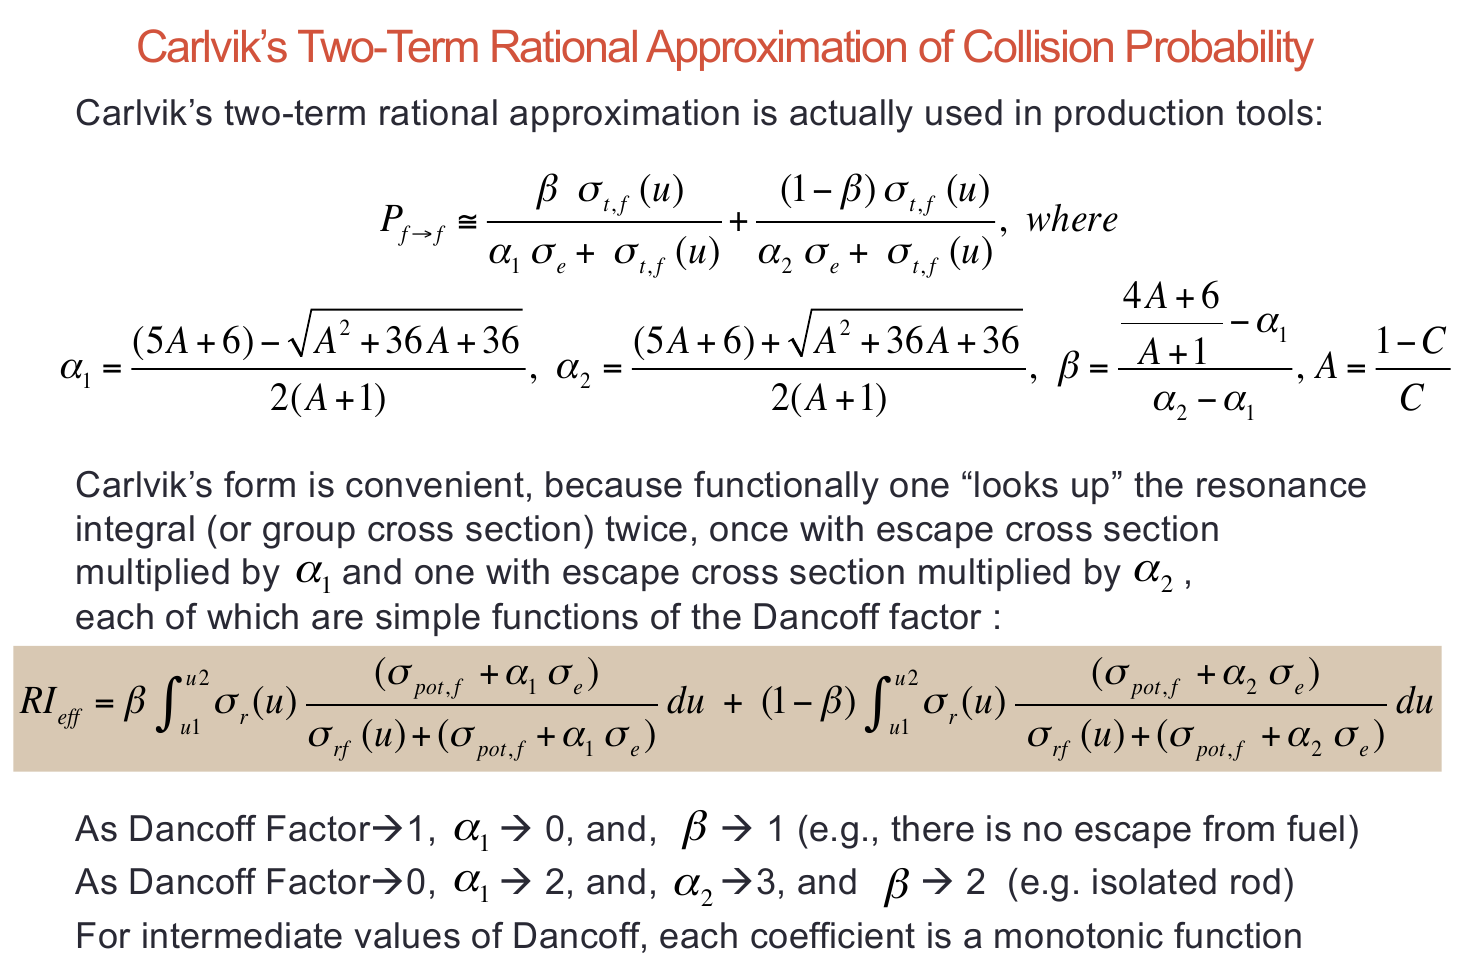
\includegraphics[width=4in]{images/r-m/Carlvik-refinement.png}
  \caption{Definition and Properties of Calvik's Refinement} \label{Calvik}
\end{figure}

Carlvik's two-term approximation is what is actually used in production tools nowaday. To use it, we essentially look up the resonance integral (or group xs) twice, once with $\sigma_e$ multiplied by $\alpha_1$ and the second time with $\sigma_e$ multiplied by $\alpha_2$, each of them are simple functions of the Dancoff factor. To double check, we let Dancoff factor to go to 1, and there should be no escape from the fuel; let Dancoff factor go to 0, we should get isolated rod. 

\end{enumerate}

\end{document}
